\documentclass[a4paper]{article}

\usepackage{caption}
\usepackage{listings}
\usepackage{fancyhdr}
\usepackage[top=3cm,bottom=3cm,left=3cm,right=3cm]{geometry}
\usepackage{color}
\usepackage{amsmath}
\usepackage{graphicx}
\usepackage{tabulary}
\usepackage{siunitx}

\definecolor{dkgreen}{rgb}{0,0.6,0}
\definecolor{gray}{rgb}{0.5,0.5,0.5}
\definecolor{mauve}{rgb}{0.58,0,0.82}

\lstset{frame=tb,
  language=Octave,
  aboveskip=3mm,
  belowskip=3mm,
  showstringspaces=false,
  columns=flexible,
  basicstyle={\small\ttfamily},
  numbers=none,
  numberstyle=\tiny\color{gray},
  keywordstyle=\color{blue},
  commentstyle=\color{dkgreen},
  stringstyle=\color{mauve},
  breaklines=true,
  breakatwhitespace=true,
  tabsize=3
}

\newcommand{\HRule}{\rule{\linewidth}{0.5mm}}
\pagestyle{fancy}
\lfoot{\small \color{gray}Tom Peerdeman - 10266186}
\cfoot{\thepage}
\rfoot{\small \color{gray}Ren\'e Aparicio Sa\'ez - 10214054}
\lhead{\small \color{gray}Autonome Mobiele Robots}

\begin{document}
\begin{titlepage}
\begin{center}
\textsc{\Large Autonome Mobiele Robots}\\[0.5cm]
\HRule \\[0,4cm]
\textsc{\huge \bfseries NXT - Particle filter based simultaneous localization and mapping}
\HRule \\[8cm]
\begin{minipage}{0.4\textwidth}
\begin{flushleft}\large
\emph{Auteurs: Tom Peerdeman \& Ren\'e Aparicio Saez}\\
\end{flushleft}
\end{minipage}
\begin{minipage}{0.4\textwidth}
\begin{flushright}\large
\emph{Datum: \today\\\hspace{1cm}}\\
\end{flushright}
\end{minipage}
\end{center}
\end{titlepage}

\tableofcontents
\newpage

\section{Materiaal}
Om de experimenten uit dit rapport te kunnen uitvoeren zijn de volgende materialen gebruikt:\\
- PC/Laptop met Matlab\\
- Boek: Autonomous Mobile Robots 2th Edition - Roland Siegwart et al.\\
- NXT-Robot\\
- Logitech Webcam\\
- Gloeilamp\\
- Zwarte tape

\section{Introduction}
Een autonome mobiele robots moet een kaart kunnen opbouwen van zijn omgeving. Aan de hand van zijn eigen gemaakte kaart zou hij met behulp van bekende kaarten kunnen bepalen waar hij zich in de wereld bevindt. Een veel gebruikte methode om een kaart al rijdend op te bouwen is SLAM (Simultaneous Localization And Mapping). Er kan dan met een bepaalde zekerheid bepaald worden waar de robot zich momenteel bevindt. Het is de bedoeling dat de robot in een gebied rond kan rijden en hierbij een goede kaart kan maken. Zo moet hij bijvoorbeeld na het rijden van een rondje weer hetzelfde deel van de kaart zien (mits er niks veranderd is aan de omgeving).

\section{Feature detection}
De gebruikte versie van SLAM, fastSLAM, maakt gebruik van ruwe odometrie data en features welke gedetecteerd worden door de laserscan.
Als feature zal gebruik gemaakt worden van hoeken van lijnen. Om de corners te kunnen vinden zullen eerst de lijnen gevonden moeten worden uit de ruwe punten data die de laserscan aanlevert. Om deze lijnen te kunnen detecteren wordt gebruik gemaakt van het split \& merge algoritme. Het split en merge algoritme is in stappen uitgelegd in listing \ref{lst:splitmerge}.

\begin{lstlisting}[caption= Split \& merge algorithm, label=lst:splitmerge, numbers=left]
Initially: set s1 consists of all N points. Insert s1 to the list L. Set index i=1
Fit a line to the next set si in L
Detect the point P with the maximum distance D to the line
if D is less than a threshold then continue to step 2
else split si at P into si1 and si2, replace si , in L, by si1 and si2. Continue to step 2
When all sets (segments) in L have been checked, merge collinear segments.
\end{lstlisting}

\noindent Het fitten van een lijn wordt hierbij gedaan door het zoeken naar een lijn zodanig dat de som van de afstanden in het kwadraat van de punten tot de lijn minimaal is. De lijn wordt hierbij uitgedrukt in polaire co\"ordinaten $r$ en $\alpha$ (zie figuur \ref{fig:linefit}). 
Dat is dus als de formule $D^2 = \sum\limits_{i=1}^n r-x_i cos(\alpha) - y_i sin(\alpha)$ minimaal is. Om de waardes van $r$ en $\alpha$ te kunnen vinden kunnen we dan gebruik maken van de afgeleiden. Oftewel $\frac{d(D^2)}{dr} = 0$ en $\frac{d(D^2)}{d\alpha} = 0$.
We krijgen hieruit de vergelijkingen:\\
$nom =  -2\sum\limits_{i=1}^n (x_i - x_c)(y_i - y_c)$\\
$dennom =  \sum\limits_{i=1}^n (y_i - y_c)^2 - (x_i - x_c)^2$\\
$\alpha = 0.5\mbox{ atan2}(nom, denom)$\\\\
Hierbij zijn $x_c$ en $y_c$ de co\"ordinaten van het middelpunt van alle punten. Hiervoor nemen we simpelweg het gemiddelde van de $x$ dan niet de $y$ waardes van alle punten. Aan de hand van de $\alpha$ parameter kunnen we de $r$ parameter vinden.
Het is namelijk zo dat een punt op een lijn uitgedrukt in polaire co\"ordinaten voldoet aan de vergelijking $x cos(\alpha) + y sin(\alpha) = r$. We kunnen hiermee de $r$ parameter vinden als we een punt weten dat zeker op de lijn ligt. Dit punt is....
% WELK PUNT???

Als we nu naar de punten kijken die het verste op de lijn liggen kunnen we de uiteindes van dit lijnsegment bepalen. Het wordt nu ook makkelijk om hoeken te zoeken door alleen naar deze uiteindes te kijken en zien of ze een hoek vormen met een ander lijnsegment. 

\begin{figure}[h]
	\centering
	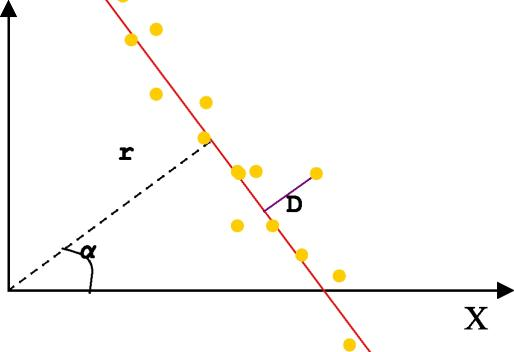
\includegraphics[width=0.7\textwidth]{img/stolenline.png}
	\caption{Fitten van de lijn door de som van D kwadraat te minimaliseren}
	\label{fig:linefit}
\end{figure}

\section{fastSLAM algoritme}
Het fastSLAM algoritme maakt gebruik van particles. Hierbij kan elk particle voorgesteld worden als een kans dat de robot aanwezig is op de positie van de robot, de stand van de robot maakt hierbij ook deel uit van de positie. Het algoritme werkt met twee stappen.\\
Stap 1 is de odometrie update. In deze stap wordt gekeken naar de verplaatsing van de robot. Aan de hand van de encoderwaardes kan worden uitgerekend welke afstand gereden is. Aangezien de kans op een verschil tussen de gemeten waarde en de echt afgelegde afstand groot kunnen we voorspellen dat de particles ook met een bepaalde error zich zullen voortbewegen. Deze error wordt aangenomen gaussisch te zijn. De nieuwe positie van een particle kunnen we dan voorspellen met \\\\
$
\begin{bmatrix}
x\\
y\\
\theta
\end{bmatrix}^{t+1}
=
\begin{bmatrix}
(x_t + dr_n cos(dth_n + \theta_t))\\
(y_t + dr_n sin(dth_n + \theta_t)) \\
pi2pi(pi2pi(\theta) + dth)
\end{bmatrix}
$\\\\
Hierbij is $pi2pi$ een functie die hoeken omzet van de range $[0 2\pi]$ naar $[0,pi], (-pi, 0]$.
$dth_n$ is de toegevoegde noise voor de afgelegde hoek $dth$.
$dr_n$ is de toegevoegde noise voor de afgelegde afstand.\\
Het is belangrijk te vermelden dat er meerdere odometrie updates kunnen voorkomen voordat stap 2 uitgevoerd wordt. Hierdoor kan de error in de particle positie vrij hoog oplopen. Deze error moet dat naar beneden gebracht worden door de data uit de laserscan (stap 2).\\\\
Stap 2 is de laserscan update

\section{Deel 2, Eigen data}
\subsection{Offline SLAM met behulp van een dataset}
Er moet worden gewerkt met een offline dataset, in verband met tijdgebrek en het niet aanwezig zijn van voldoende robots. De meegeleverde dataset bestaat uit 61 fotos.
Voordat begonnen kan worden met het opbouwen van een kaart moeten eerst de parameters voor de camera worden gecalibreerd. De fotos bevatten echter twee verschillende centers. Na het 40e plaatje veranderd de center enigszins (Picture 51.jpg tot het einde van de dataset). De centers zijn respectievelijk $centre1 = [465;343]$ voor de eerste 40 fotos en $centre2=[465;335]$ voor de overige fotos. Alle fotos maken gebruik van $\alpha = 140$ en $Rmin = 100$ en $Rmax = 180$. Er is gebruik gemaakt van een BWtreshold van 100, behalve voor Picture 17.jpg tot Picture 22.jpg. Hierbij is de treshold verlaagd naar 90. Dit is gedaan omdat bij deze fotos de draad die de camera met de laptop verbind gemeten wordt. De draad beinvloed hiermee de data. In figuur \ref{fig:route} is te zien welke route gereden is.
Deze kaart met bijbehorende route zal ongeveer overeen moeten komen met de opgebouwde kaart door het SLAM algoritme.
\begin{figure}[h]
	\centering
	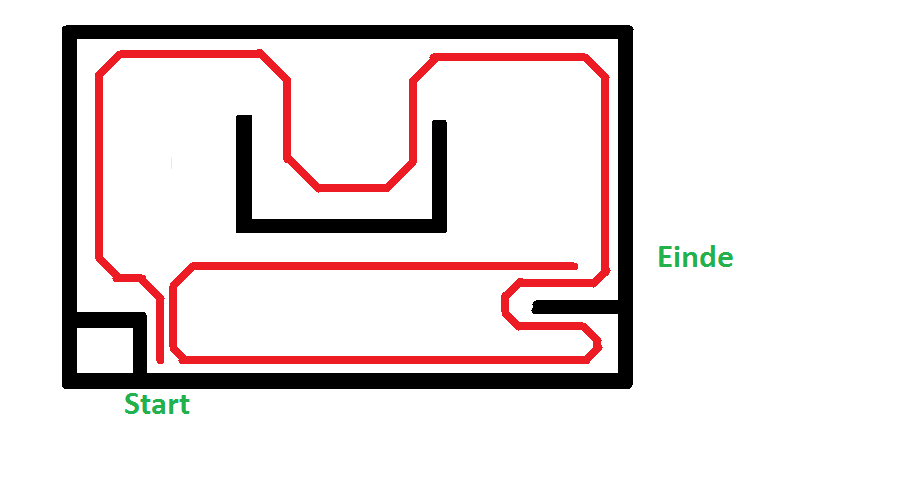
\includegraphics[width=0.7\textwidth]{matlab/imgs/route.png}
	\caption{Afgelegde route}
	\label{fig:route}
\end{figure}

\subsection{Odometrie bepalen}
Omdat er gebruik gemaakt wordt van een dataset van fotos en niet van de meegeleverde GUI, moet de odometrie met de hand worden gemaakt. Aan de hand van de meegegeven layout en het bekijken van de locatie van de robot aan de hand van de fotos kan een schatting gemaakt worden van de afgelegde afstanden.
\begin{figure}[h]
	\centering
	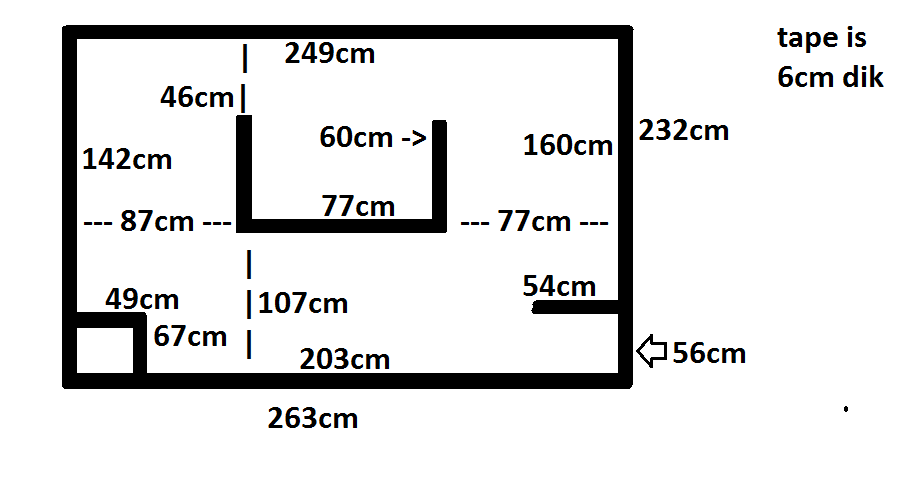
\includegraphics[width=0.7\textwidth]{matlab/imgs/layout.png}
	\caption{Layout van de kaart}
	\label{fig:layout}
\end{figure}
Deze schatting kan aan de hand van experimenten worden geoptimaliseerd. Deze optimalisatie wordt gedaan door afgelegde afstanden te vergroten of te verkleinen. In een enkel geval moet de draaihoek worden aangepast. De meeste bochten die gemaakt worden bestaan uit twee korte bochten van elk $\SI{45}{\degree}$. Er zijn echter twee bochten waarbij eerst een draaiing wordt gemaakt van $\SI{60}{\degree}$ gevolgd door een draaiing van $\SI{30}{\degree}$.
\subsection{Resultaten}
Het resultaat met geoptimaliseerde odometrie is zichtbaar in figuur \ref{fig:final}. 
\begin{figure}[h]
	\centering
	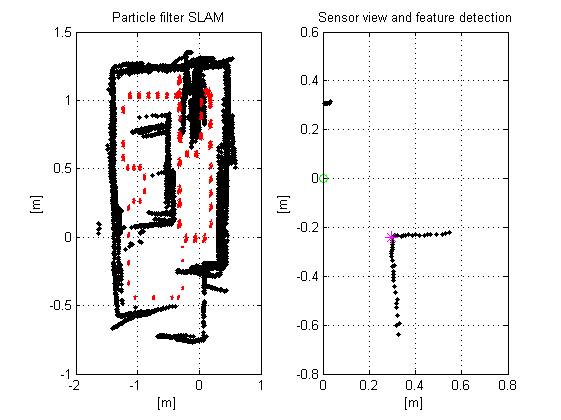
\includegraphics[width=0.7\textwidth]{img/statusnow.png}
	\caption{Uiteindelijk resultaat}
	\label{fig:final}
\end{figure}
\subsection{Discussie}
Er is ruis zichtbaar in het resultaat. Ditheeft te maken met het mogelijk nog meer te optimaliseren van de odometrie of door het optimaliseren van de parameters.
Omdat de dataset twee verschillende centers heeft, ontstaat ruis vanaf plaatje 41. Dit zorgt voor meer ruis (de dikkere muur) rechtsboven in figuur \ref{fig:final}.
\subsection{Verbeteringen}
De odometrie houdt momenteel alleen rekening met de afgelegde afstand in de huidige rijrichting van de robot. Het is hierdoor niet mogelijk om met behulp van fotos een daadwerkelijke bocht aan te geven. Het algoritme denkt nu dat er een rechte lijn wordt gereden en vervolgens wordt gedraaid, in plaats van een continue draaiing over de af te leggen afstand uit te voeren.

\end{document}
